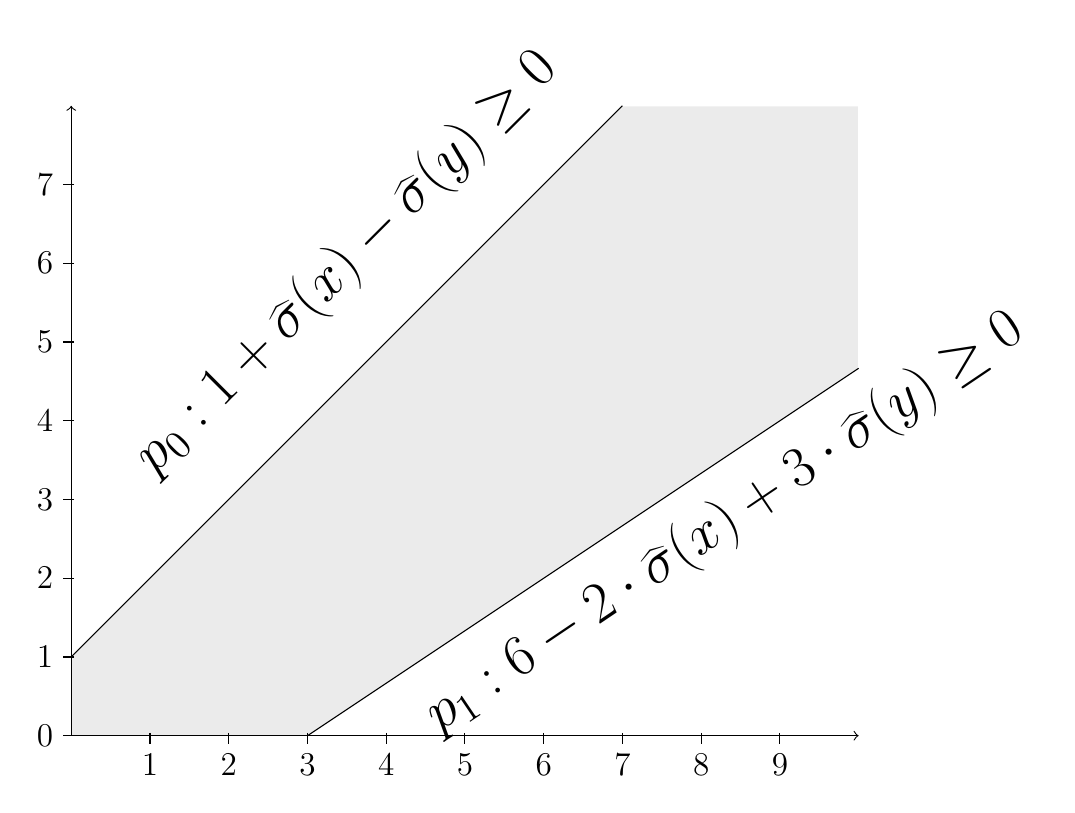
\begin{tikzpicture}[only marks]

    % Pintamos el fondo del poliedro
    \draw[color=white, fill=black!8] (0,1) -- (7,8) -- (10,8) -- (10,14/3) -- (3,0) -- (0,0);
        
    % Dibujamos los ejes
    \draw[->] (0,0) -- coordinate (x axis mid) (10,0);
    \draw[->] (0,0) -- coordinate (y axis mid) (0,8);

    % "Marcamos" los ejes
    \foreach \x in {1,2,3,4,5,6,7,8,9}
        \draw [](\x cm,1pt) -- (\x cm,-3pt)
            node[anchor=north] {\large $\x$};
    \foreach \y in {0,1,2,3,4,5,6,7}
        \draw (1pt,\y cm) -- (-3pt,\y cm) node[anchor=east] {\large $\y$};
        
    % Facetas 
    \draw[-] (0,1) -- coordinate (x axis mid) (7,8);
    \node[rotate=45] (ine1) at (3.5,6.0) {\huge $p_0:1 + \widehat\sigma(x) - \widehat\sigma(y) \geq 0$};

%    \draw[-] (7,8) -- coordinate (x axis mid) (10,8);
%    \node[] (ine2) at (11.0,8.5) {\huge $p_1:9 - \widehat\sigma(y) \geq 0$};
%
%    \draw[-] (10,8) -- coordinate (x axis mid) (10,14/3);
%    \node[] (ine3) at (13.0,6.1) {\huge $p_2:10 - \widehat\sigma(x) \geq 0$};

    \draw[-] (3,0) -- coordinate (x axis mid) (10,14/3);
    \node[rotate=34] (ine4) at (8.3,2.7) {\huge $p_1:6 -2 \cdot \widehat\sigma(x) + 3 \cdot \widehat\sigma(y) \geq 0$};
    
    
%    \node[rotate=45] (p) at (10.5,6.5) {\Huge $\dots$};     
%    \node[rotate=45] (p) at (7.5,8.5) {\Huge $\dots$};     
%    \node[rotate=45] (p) at (9.5,8.5) {\Huge $\dots$};
%               
\end{tikzpicture}
